\documentclass[tikz,border=2pt]{standalone}
\usepackage{pgfplots}
\pgfplotsset{compat=1.18}
\usetikzlibrary{intersections}
\usepgfplotslibrary{fillbetween}


\begin{document}
	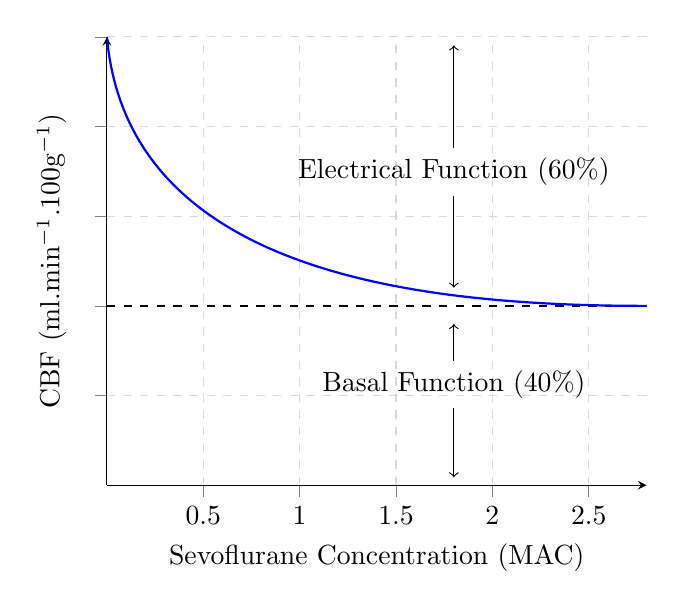
\begin{tikzpicture}
		\begin{axis}[
			axis lines=middle,
			ymin = 0,
			ymax = 5,
			xmin = 0,
			xmax= 2.8,
			grid = major,
			grid style={dashed, gray!30},
			ylabel near ticks,
			xlabel near ticks,
			xlabel= Sevoflurane Concentration (MAC),
			ylabel= CBF (ml.min$^{-1}$.100g$^{-1}$),
			tick align=outside,
			yticklabels={,,}
			legend style={font=\small, cells={align=left}}]


			\draw [black, dashed, thick] (0, 2) -- node[pos=0.6, name = mid]{} ( (3, 2);
			\draw [blue, thick] (0,5) to[out =275, in = 180] (2.8,2);

			\coordinate (o) (0,0);

			\node [below of=mid, name = basal]{Basal Function (40\%)};
			\draw [->, shorten >=1mm] (basal) -- (mid);
			\draw [->, shorten >=1mm] (basal) -- (o -| mid);
			
			\node [above of=mid, yshift = 0.7cm, name = elec]{Electrical Function (60\%)};
			\draw [->, shorten >=1mm] (elec) -- (mid);
			\draw [->, shorten >=1mm] (elec) -- +(0,1.5);

		\end{axis}
	\end{tikzpicture} 
\end{document}